\chapter{Theoretical background of thermal infrared remote sensing}

\label{Chapter2}

%description
%----------------------------------------------------------------------------------------
This chapter reviews some fundamentals of thermal remote sensing (Section 2.1), as well as a useful approach, which is also used in the MITIP method, to identify and determine target temperature of subpixle resolution (Section 2.2). \\

%----------------------------------------------------------------------------------------
%	SECTION 1
%----------------------------------------------------------------------------------------

\section{Principles of thermal infrared remote sensing}
Thermal remote sensing depends on the fact that any object with a temperature above absolute zero (0 K or -273.15 $^\circ$C) emits electromagnetic (EM) radiation in the infrared range. For example, the Earth we live has an average temperature around 300 K and its peak emittance is near 10 $\mu$m, which falls on thermal infrared (TIR) domain \parencite {Reference201, Reference202}. The spectral composition and intensity of the emited radiation are determined by its surface temperature, which is also called kinetic temperature $T_{kin}$,  and the emissivity of the object \parencite{Reference207}. The emissivity $\epsilon_{\lambda}$, $\epsilon$ for short, is a ratio of the radiant flux of an object at a certain temperature to the radiant flux of a blackbody at the same temperature, representing the effectiveness of the object in emitting energy as thermal radiation. The blackbody is an idealized physical object that aborbs and re-emits all incident EM radiation, which means its emissivity is 1 \parencite{Reference206, Reference204}. The emissivity varies as a function of wavelength $\lambda$ and also depends on the surface type of the object, but is not temperature-dependent \parencite{Reference203}.\\

% Thus these sensors will produce thermal radiance images which record the equivalent blackbody radiances of the object on the Eearth's surface 
\noindent The satellite remote sensing snesors responsive in the thermal infrared domain are capable to record the EM radiations emited by Earth surface objects \parencite{Reference204}. With the recorded radiation the derivation of the radiant temperature $T_{rad}$ is possible. Radiant temperature $T_{rad}$ is the actual temperature obtained from the measurement of the sensor, representing temperature of a equivalent blackbody \parencite{Reference206}. Notice that the radiant temperature $T_{rad}$ and the kinematic temperature $T_{kin}$ are two different terms and the conversion between them will be introduced later.\\

%-----------------------------------
%	SUBSECTION 1
%-----------------------------------

\subsection{The thermal infrared  domain and atmospheric windows}
There is no strict or physical definition of the thermal infrared domain. Usually the thermal infrared wavelength domain spread from around 3 to 14 $\mu$m. Within this range, there are two atomspheric windows in the 3 - 5 $\mu$m range and in the 8 - 14 $\mu$m range \parencite{Reference204}. \\

\begin{figure}[!htbp]
  \centering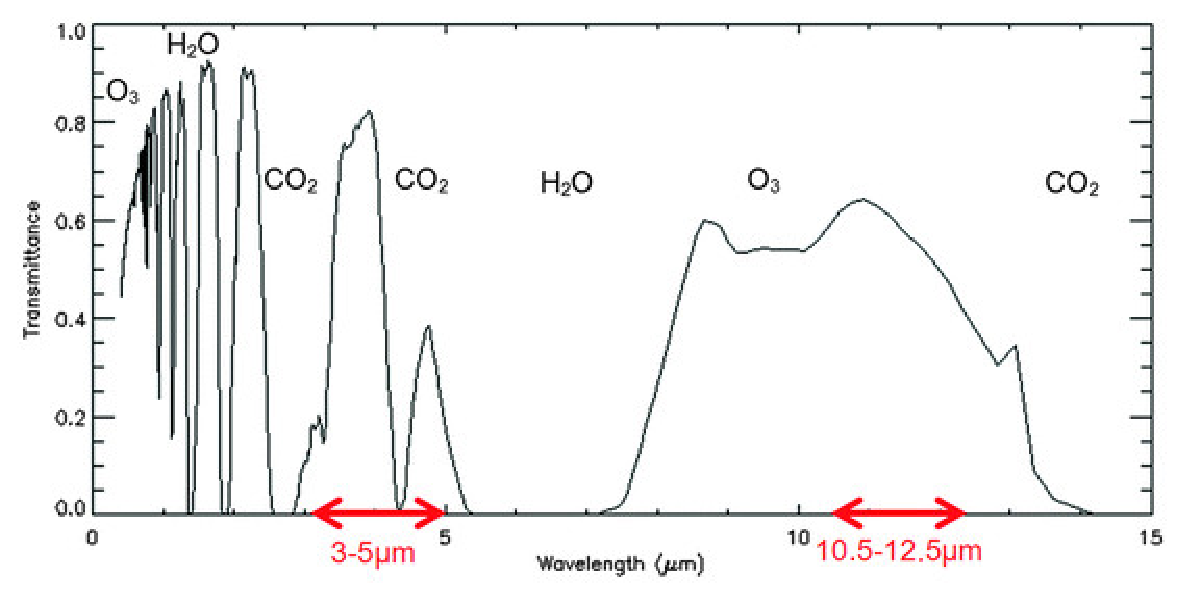
\includegraphics[width=0.8\textwidth]{The_thermal_infrared_wavelength_domain.eps}
  \caption{The thermal infrared wavelength domain \parencite{Reference204}.}
  \label{fig:TIRdomain}
\end{figure}

\noindent The spectrum range 8 - 14 $\mu$m, which is called Long-Wavelength InfRared (LWIR), is the thermal imaging region. Within this range, sensors are able to obtain a completely passive image of objects based on the thermal emissions only and no illumination required. There is only a absorption of OZone which might merely neglected by the sensor. The sepectrum range 3 - 5 $\mu$m is called Mid-Wavelength InfraRed (MWIR). Sensors responsive to this specturm range will capture reflected sunlight which contaminates the object-emitted thermal signal. So More attention should be paid when dealing with day-time 3 - 5 $\mu$m MWIR imagery. \\

\noindent In this thesis, we will focus on the night-time TET-1 imagery only. \\

%-----------------------------------
%	SUBSECTION 2
%-----------------------------------

\subsection{The Planck's law and Stefan-Boltzmann law}

%----------------------------------------------------------------------------------------
%	SECTION 2
%----------------------------------------------------------------------------------------

\section{A dual-channel method for the identification of subresolution high temperature sources}

%----------------------------------------------------------------------------------------
%	SECTION 3
%----------------------------------------------------------------------------------------

%\section{The mitip, an atmospheric correctoin and image processing method}